\section{Implementation of a swarm system \label{Appendix:RobotSystem}}

There are several reasons to realise a swarm system:
\begin{enumerate}
 \item proof of concept
 \item technology showcase during open events
 \item solve a business task
\end{enumerate}
Software simulations don not take into account the complexity of the real world
and uncertainty introduced by mechatronic systems, therefore a real implementation
 is likely to spot unexpected behaviour of the system.
A live swarm system can be used to sponsor research and attract new students/researchers
 in this area and is also fun to watch.
Additionally it can be extended to solve real business tasks, for example the
company ``Kiva Systems'' used a swarm system to improve the performance
of order fulfilment \footnote{The company website is: http://www.kivasystems.com/index.html}.
Nevertheless there are 3 main challenges:
\begin{itemize}
 \item scaling down the costs for large systems
 \item operating conditions
 \item replicability
\end{itemize}
A swarm systems is likely composed of many agents, otherwise it doesn't make
sense to call it a swarm: therefore the price of every single unit must be very low.
Hence the unit must have different hardware according to the task it was designed for:
if the task is to move boxes we need grip actuators to move them and
cameras to determine their location.
I designed my system to be easy to replicate on the hardware and software side,
this is important for other researchers if they want to test new algorithms or
replicate the results.
The robots/agents are positioned on a rectangular playground with a white background,
 a food patch is painted in the centre as a graded circle. The robots must have
reflective sensors pointing down to detect food signals, contact sensors to avoid
each other as well as walls and a communication method to exchange information.
\subsection{The playground}
The playground is printed on a grey scale A3 paper. The playground dimensions
are reported in the figure. The robot we are using, called 3pi, from Pololu has the
 same diameter has the inner black spot.
The background and the wall are at high contrast white/black and the blob at the
centre has a gradient texture: the robot will pass over it to calibrate the minimum,
maximum and average readings from its reflective sensors looking down to the floor.
\begin{figure}[htbp]
\begin{center}
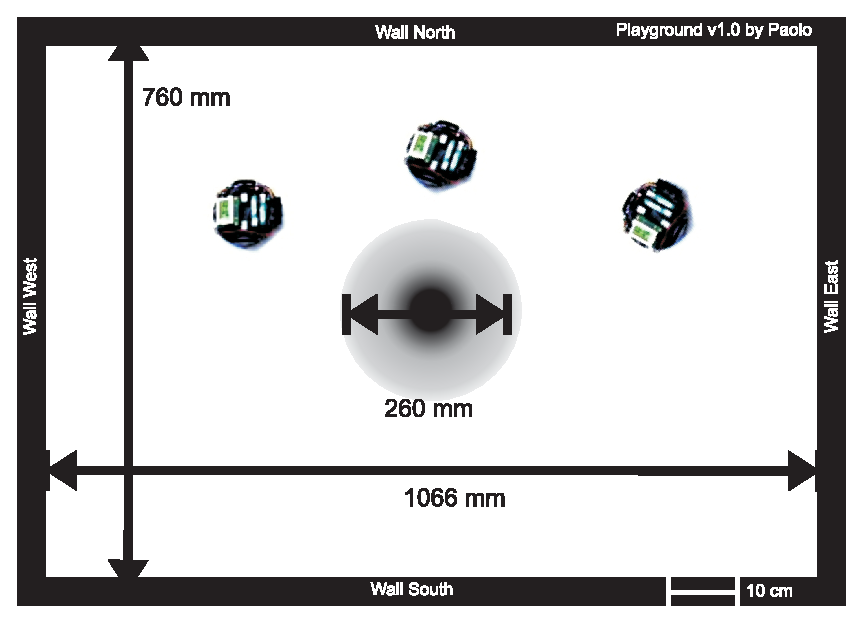
\includegraphics[scale=0.8]{figures/playground/playgrounddesc.eps}
\caption[Playground setup]{The playground dimensions}
\end{center}
\end{figure}
\subsection{Hardware platform and software development}
There were two main choices about the hardware implementation:
\begin{itemize}
 \item custom design: designing the electronic and mechanical part
\begin{itemize}
\item advantages: total control on choice of processor, sensors, actuators, communication
\item disadvantages: manufacturing can become an issue: assembly errors, testing and labour cost. Not easy to be used by external researchers, documentation and materials must be provided but mechanical parts are easy to find etc...
\end{itemize}
 \item open design:
\begin{itemize}
\item advantages: available virtually to everybody, easy to use and to obtain
\item disadvantages: limited control on the hardware
\end{itemize}
\end{itemize}

According to the table above I decided to use 2 commercial popular robots so that virtually everybody can use them and replicate my results. The first choice is the lego mindstorm nxt which was released by Lego as a fully open source documented platform on 1 May 2006. Lego \nomenclature{Lego}{A company producing modular robotic kits} sold 150,000 units in 2007 worldwide. The second choice is the 3pi from Pololu (see specifications here \ref{Pololu}).
I have chosen these two because they are in a different price range (£150 and $\$60$ respectively) and have a different hardware complexity.
To simplify the software development I:
\begin{enumerate}
 \item developed a common C++ library called UICO
 \item compiled, tested and debugged under x86 (a common desktop pc)
 \item adapted to the programming environments of the lego nxt and pololu 3pi
 \item verified again the program behaviour in the real application
\end{enumerate}

All the libraries I developed are available on-line and can be easily installed and compiled by any other user.


\subsection{Lego NXT mindstorm}
Lego has 10 years experience in producing educational robot kits, NXT\footnote{http://mindstorms.lego.com/} is an updated version of the RCX\footnote{http://www.lego.com/eng/education/mindstorms/home.asp?pagename=rcx} kit. With this product Lego has released full hardware and software specification of the kit\footnote{http://mindstorms.lego.com/eng/Overview/nxtreme.aspx} so that users can develop their own firmware and interface different hardware NXT controller.
\begin{figure}[htbp]
\begin{center}
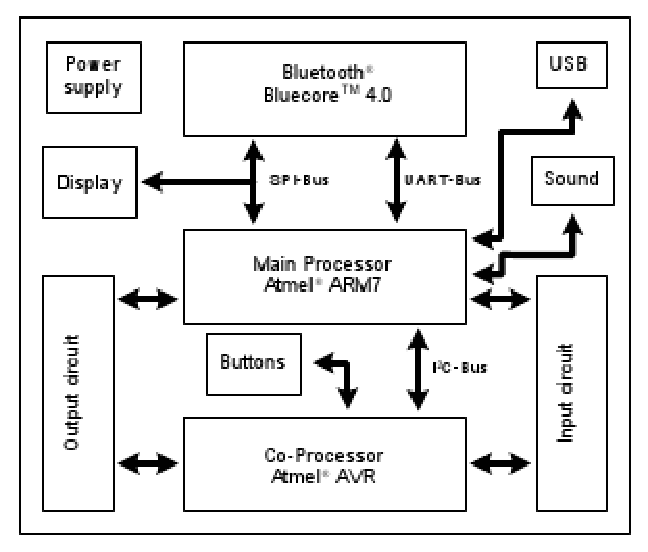
\includegraphics[scale=0.6]{figures/legonxt/nxthardware.eps}
\caption[Lego NXT robot implementation]{Hardware block diagram of the NXT brick. For a better description see Appendix \ref{LegoNxt}}
\end{center}
\end{figure}
Recently Professor Masaaki Mizuno (Department of Computing and Information Sciences, Kansas State University) did a port of the TOPPERS/ATK to the NXT naming it \textbf{nxtOSEK}.
\textbf{nxtOSEK }\footnote{http://lejos-osek.sourceforge.net/}\ consists of device driver of  leJOS NXJ C/Assembly source code, TOPPERS/ATK (Automotive Kernel, formerly known as TOPPERS/OSEK) and TOPPERS/JSP Real-Time Operating System source code that includes ARM7 (ATMEL AT91SAM7S256) specific porting part, and glue code to make them work together. nxtOSEK can provide:

\begin{itemize}
\item ANSI C/C++ programming environment by using GCC tool chain

    \item C API for NXT Sensors, Motor, and other devices
    \item C++ API for NXT Sensors and Motor which include many third party sensors
    \item TOPPERS/ATK provided real-time multi tasking features proven in automotive industry
    \item TOPPERS/JSP provided real-time multi tasking features that complied with Japan original open RTOS specification $\mu ITRON 4.0$
    \item Fast execution and less memory consumption
    \item There are three ways to upload the nxtOSEK application to the NXT
     \begin{enumerate}
	\item  Using John Hansen's Enhanced NXT firmware
		(multiple nxtOSEK programs can be uploaded to a NXT. However, a nxtOSEK program has to be less than 64Kbytes)
	\item Using NXT BIOS (max. 224Kbytes single nxtOSEK program uploaded to Flash)
	\item Direct boot from RAM (max. 64Kbytes single nxtOSEK program uploaded to RAM, no Flash write)
	\end{enumerate}
    \item Many examples (including NXTway-GS and NXT GT...)
\end{itemize}


\begin{figure}[htbp]
\begin{center}
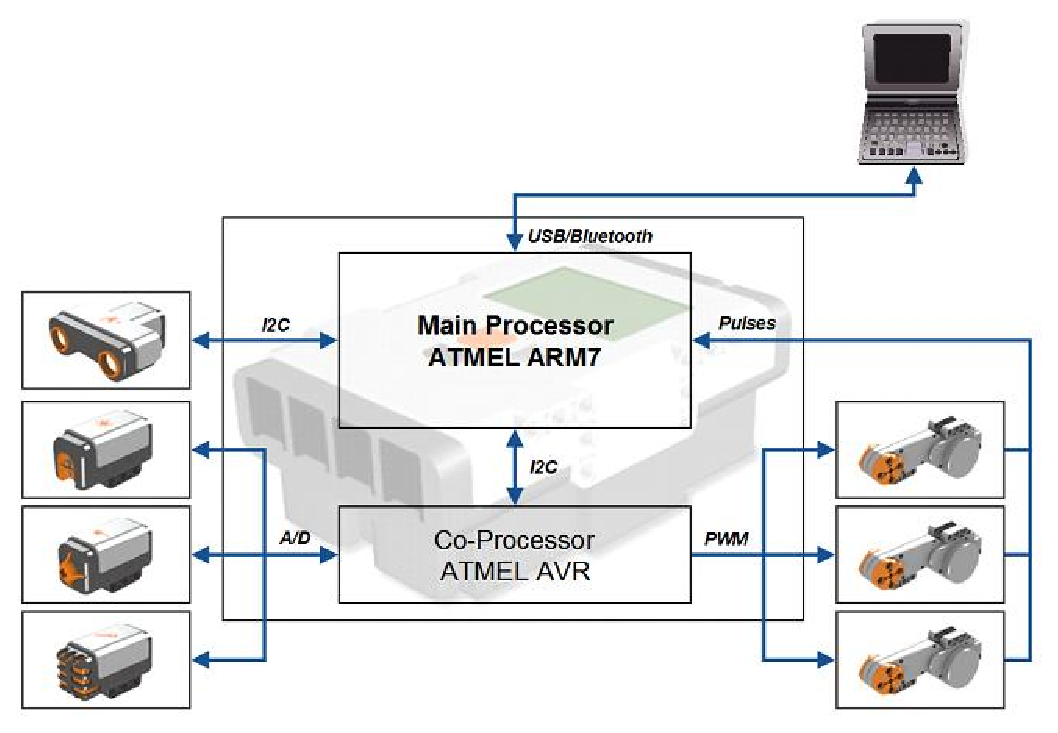
\includegraphics[scale=0.6]{figures/legonxt/nxtsystem.eps}
\caption[ATMEL AVR architecture]{This figure tells that communication between the main ARM7 processor (ATMEL AT91SAM7S256) and Sensors/Servo Motors is done via the co-processor (ATMEL AVR) except for the Ultrasonic Sensor and acquisition of Servo Motor revolutions. For nxtOSEK, the most important factor to access Sensors/Servo Motors is the communication with the co-processor via I2C serial bus. This system architecture definitely influences the software run-time environment of nxtOSEK. The main ARM7 processor accesses Sensors (to read sensor A/D value) and Servo Motors (to set PWM duty ratio and break mode) independently every 2 msec through a 1 msec periodical Interrupt Service Routine (ISR) of LEJOS NXJ platform. Servo Motors revolutions are directly captured by pulse triggered ISRs of LEJOS NXJ platform. Ultrasonic Sensor has its brain directly communicate with the main ARM7 processor via another I2C communication channel. TOPPERS ATK is similar to the following version of OSEK OS/OIL according to the TOPPERS project.
nxtOSEK restricts several TOPPERS ATK features due to the system architecture. User should not use ISR definitions and Interrupt handling API \footnote{Image and description from  http://lejos-osek.sourceforge.net/}.}
\end{center}
\end{figure}

The robot has been built using lego technic pieces from the kit: it has 2 motors with rubber wheels and a casting wheel on the back to allow differential steering. Two reflective sensors are placed on the bottom to detect food sources. Two contact sensors are placed on the front so that the robot can avoid walls and other robots.

\begin{figure}[ht]
  \begin{center}
	\subfigure[LegoRobot bottom view: left and right light sensors]{
	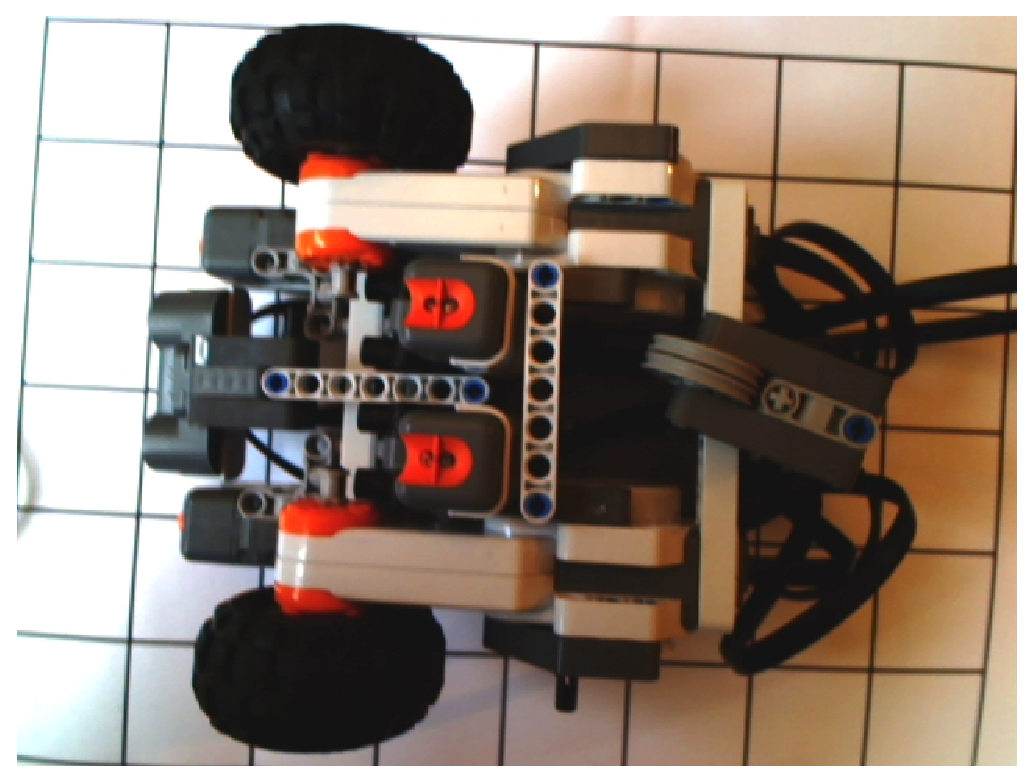
\includegraphics[scale=0.35]{figures/legonxt/legobottom.eps}}
	\hspace{1pt}
      %	\subfigure[LegoRobot up view: left and right contact senros and LCD display]{
%	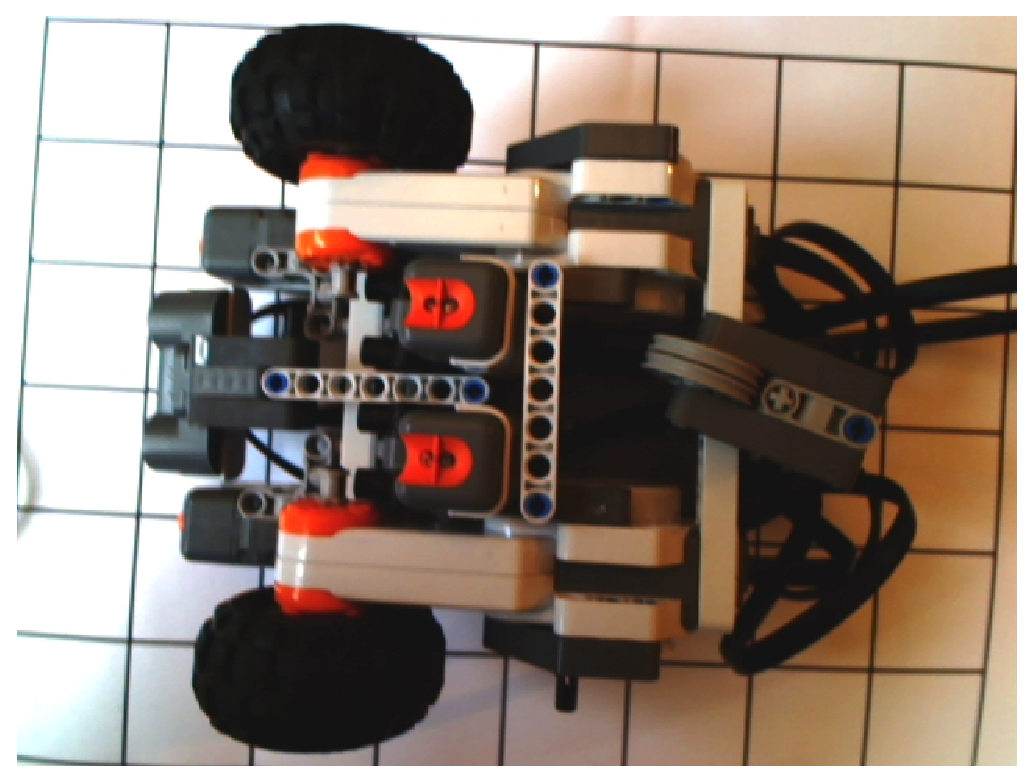
\includegraphics[scale=0.35]{figures/legonxt/legobottom.eps}}
  \end{center}
\end{figure}
The control program of the robot is using the already mentioned UICO library, and is composed of 4 tasks. They are scheduled using rate-monotonic full-preemptive scheduling (RMS): a scheduling algorithm used in real-time operating systems with a static-priority scheduling class.
The static priorities are assigned on the basis of the cycle duration of the job: the shorter the cycle duration is, the higher the job priority. In the diagram the higher priority 4 is assigned to the Control task with a 10 mseconds period, then in ascending order priority 3 to the Avoid Task, priority 2 to the DataLog task and priority 1 to the LCD task.

\subsection{Toppers}
TOPPERS\footnote{http://www.toppers.jp/en/index.html} is an acronym for “Toyohashi OPen Platform for Embedded Real-time Systems”. “Toyohashi” is a city located in Japan, and the name was selected based on project leader Professor Takada’s association with Toyohashi University of Technology when the project was started.
It is based on Open Source and Free Software and thus easy to port on any
embedded platform.

\subsection{OSEK}

OSEK/VDX is a joint project of the automotive industry. It aims at an industry standard for an
open-ended architecture for distributed control units in vehicles.
The specification of the OSEK operating system represents a uniform environment which
supports efficient utilisation of resources for automotive control unit application software. The
OSEK operating system is a single processor operating system meant for distributed
embedded control units.
One of the goals of OSEK is to support the portability and re-usability of application software.
Therefore the interface between the application software and the operation system is defined
by standardised system services with well-defined functionality. Use of standardised system
services reduces the effort to maintain and to port application software and development cost.
This is why it was so easy to port OSEK onto the Lego NXT plaftorm.
\begin{figure}[htbp]
\begin{center}
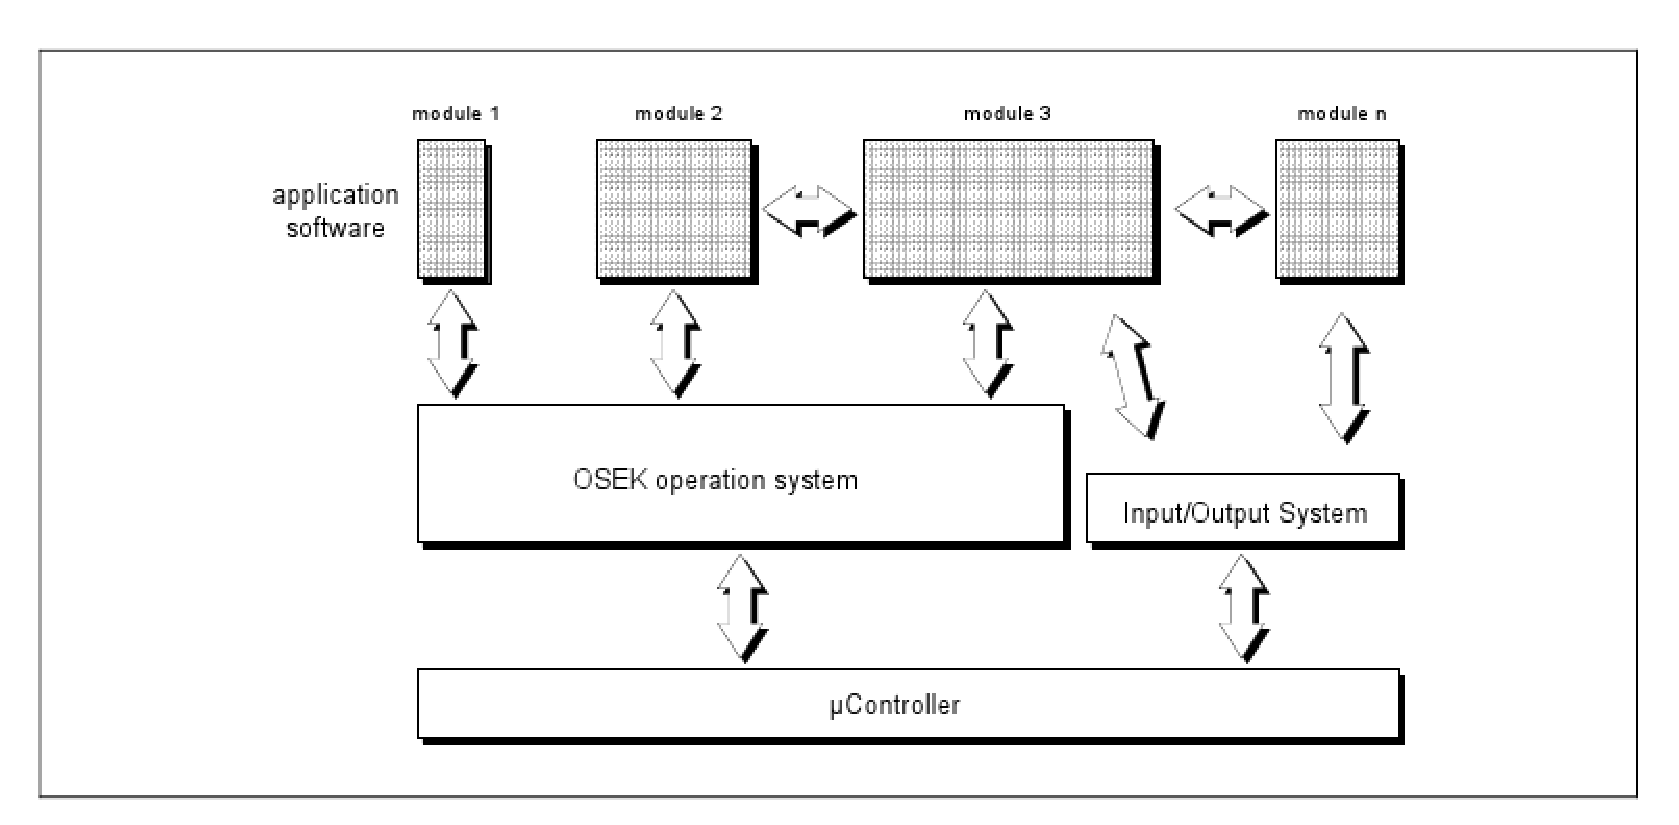
\includegraphics[scale=0.4]{figures/nxtosek/osek1.eps}
\caption{Software interfaces inside ECU}
\end{center}
\end{figure}
The OSEK operating system serves as a basis for application programs which are independent
of each other, and provide their environment on a processor. The OSEK operating system
enables a controlled real-time execution of several processes which appear to run in parallel.
The OSEK operating system provides a defined set of interfaces for the user. These interfaces
are used by entities which are competing for the CPU. There are two types of entities:
\begin{enumerate}
\item Interrupt service routines managed by the operating system.
\item Tasks (basic tasks and extended tasks).
\end{enumerate}

The hardware resources of a control unit can be managed by operating system services. These
operating system services are called by a unique interface, either by the application program or
internally within the operating system.
OSEK defines three processing levels:
\begin{itemize}
\item  Interrupt level
\item Logical level for scheduler
\item Task level
\end{itemize}

\begin{figure}[htbp]
\begin{center}
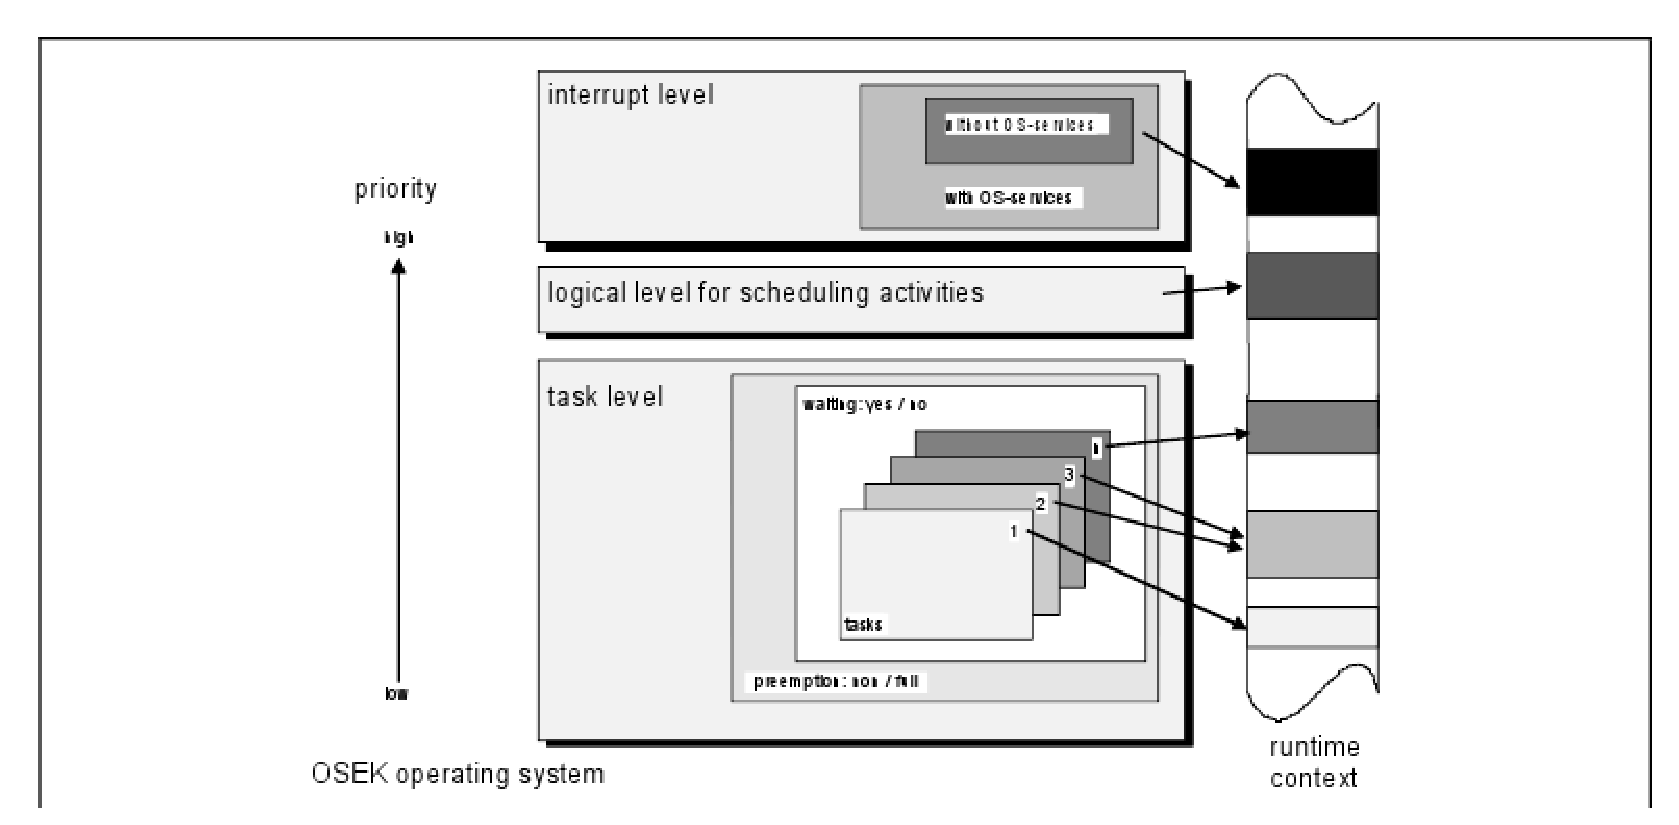
\includegraphics[scale=0.4]{figures/nxtosek/osektask.eps}
\caption{Processing levels of the OSEK operating system}
\end{center}
\end{figure}
For better portability of application software, the OSEK defines a language for a standardised
configuration information. This language "OIL" (OSEK Implementation Language) supports a
portable description of all OSEK specific objects such as "tasks" and "alarms" etc.
Website: http://www.osek-vdx.org/
\subsection{OIL}
To reach the OSEK goal of portable software, a way has been defined to describe the
configuration of an application using OSEK.
This specification only addresses a single central processing unit (CPU) in an electronic control
unit (ECU\footnote{Engine Control Unit}), not an ECU network.
\begin{figure}[htbp]
\begin{center}
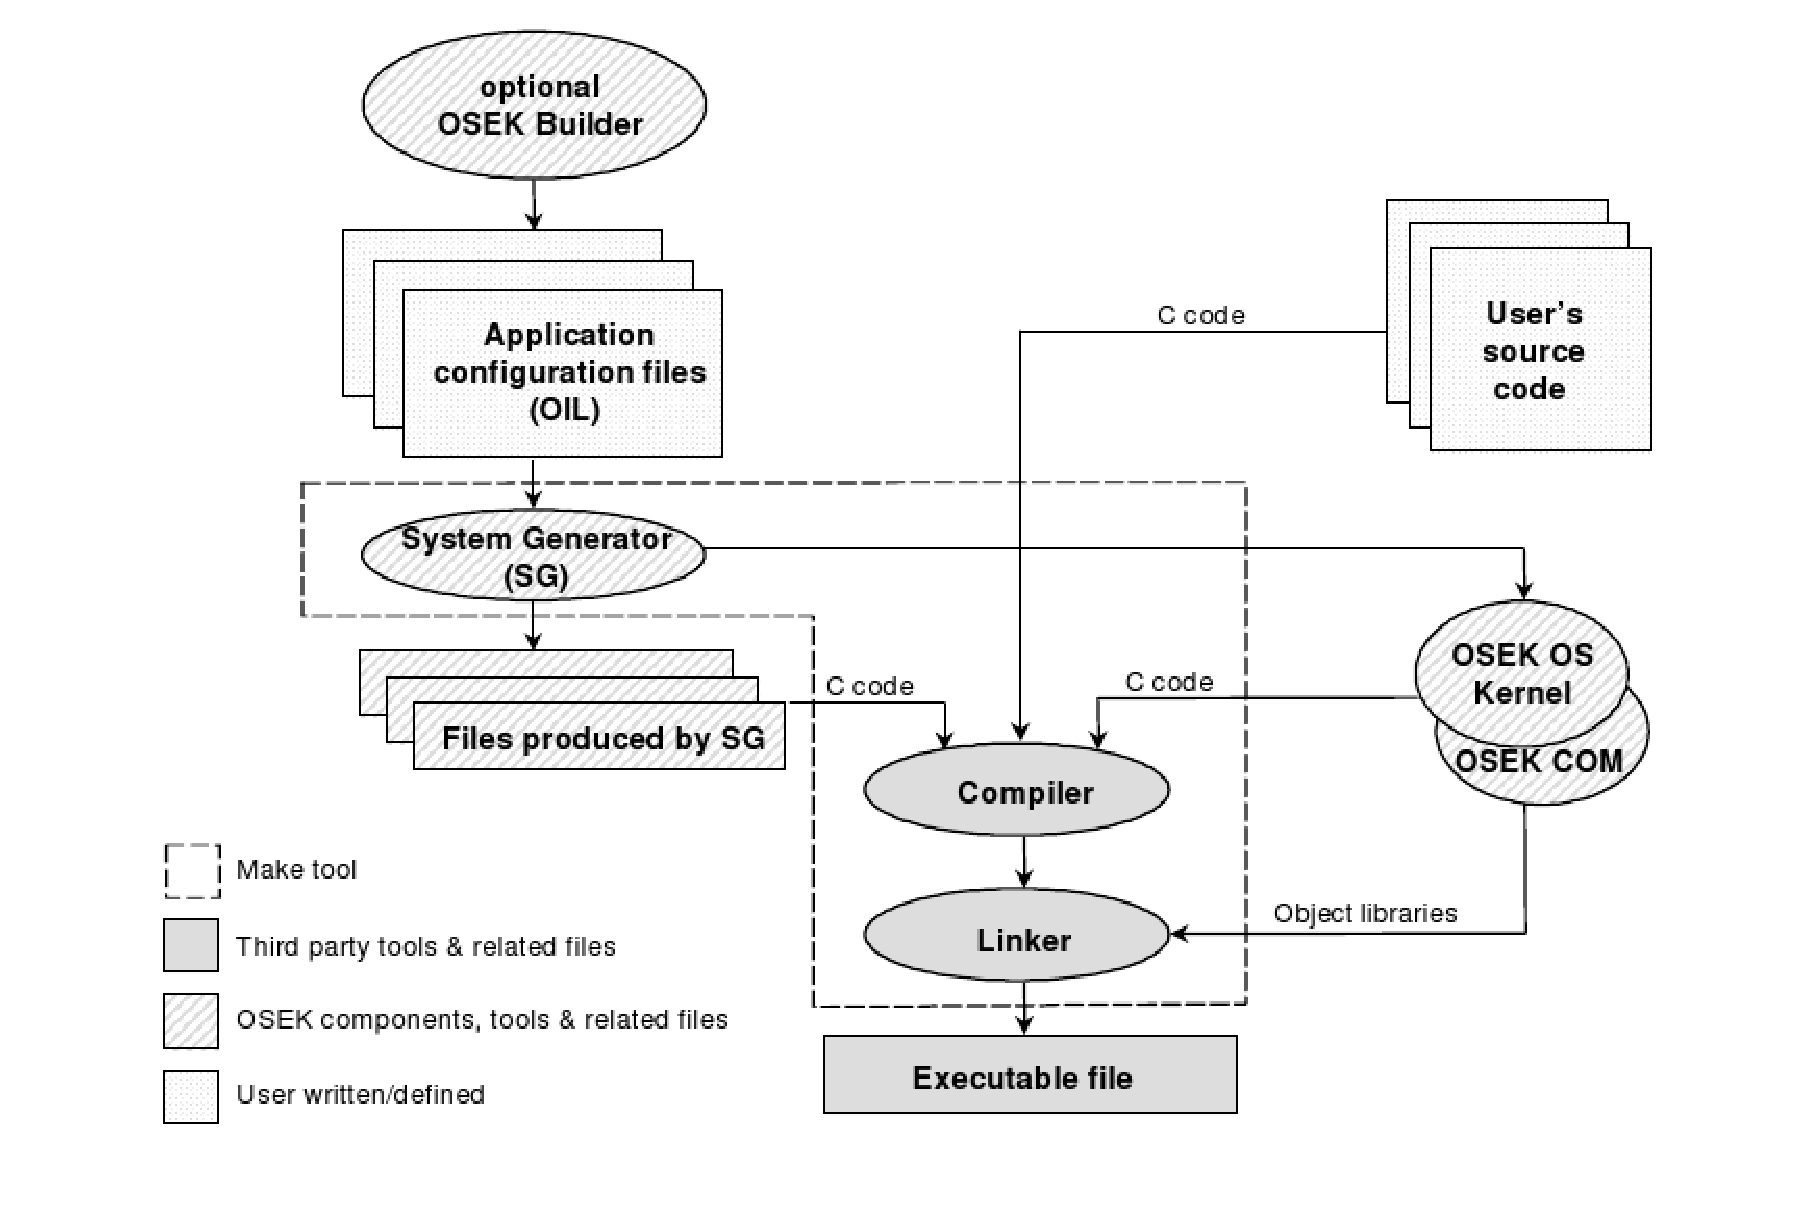
\includegraphics[scale=0.4]{figures/nxtosek/oil1.eps}
\caption{Example of development process for applications}
\end{center}
\end{figure}
The goal of OIL is to provide a mechanism to configure an OSEK application inside a
particular CPU. This means for each CPU there is one OIL description.
All OSEK system objects are described using OIL objects.
The OIL description of the OSEK application is considered to be composed of a set of OIL
objects. A CPU is a container for these OIL objects.
OIL defines standard types for its objects. Each object is described by a set of attributes and
references. OIL defines explicitly all standard attributes for each OIL object.
Each OSEK implementation, like nxtOsek, can define additional implementation-specific attributes and
references.
The OIL configuration I'm using in my robots:
\begin{small}
\begin{lstlisting}
#include "implementation.oil"

CPU ATMEL_AT91SAM7S256
{
  OS LEJOS_OSEK
  {
    STATUS = EXTENDED;
    STARTUPHOOK = FALSE;
    ERRORHOOK = FALSE;
    SHUTDOWNHOOK = FALSE;
    PRETASKHOOK = FALSE;
    POSTTASKHOOK = FALSE;
    USEGETSERVICEID = FALSE;
    USEPARAMETERACCESS = FALSE;
    USERESSCHEDULER = FALSE;
  };

  /* Definition of application mode */
  APPMODE appmode1{};

  EVENT SensorEventMask {
    MASK = AUTO;
  };

  EVENT SleepEventMask {
    MASK = AUTO;
  };


  /* Show status information */
  TASK TaskLCD
  {
	AUTOSTART = TRUE {
	APPMODE = appmode1;
	};
    EVENT = SensorEventMask;
    EVENT = SleepEventMask;
    PRIORITY = 1; /* Smaller value means lower priority */
    ACTIVATION = 1;
    SCHEDULE = FULL;
    STACKSIZE = 512; /* Stack size */
  };

   TASK TaskDataLog
  {
	AUTOSTART = TRUE {
	APPMODE = appmode1;
	};
    EVENT = SensorEventMask;
    EVENT = SleepEventMask;
    PRIORITY = 2; /* Smaller value means lower priority */
    ACTIVATION = 1;
    SCHEDULE = FULL;
    STACKSIZE = 512; /* Stack size */
  };

   TASK TaskAvoid
  {
	AUTOSTART = TRUE {
	APPMODE = appmode1;
	};
    EVENT = SensorEventMask;
    EVENT = SleepEventMask;
    PRIORITY = 3; /* Smaller value means lower priority */
    ACTIVATION = 1;
    SCHEDULE = FULL;
    STACKSIZE = 512; /* Stack size */
  };

  /* Reak time task with the digital controller */
  TASK TaskControl
  {
	AUTOSTART = TRUE {
	APPMODE = appmode1;
	};
    EVENT = SensorEventMask;
    EVENT = SleepEventMask;
    PRIORITY = 4; /* Smaller value means lower priority */
    ACTIVATION = 1;
    SCHEDULE = FULL;
    STACKSIZE = 512; /* Stack size */
  };



  TASK SensorMonitorTask {
    AUTOSTART = FALSE;
    PRIORITY = 1;
    ACTIVATION = 1;
    SCHEDULE = FULL;
    STACKSIZE = 512;
  };

  /* Definition of OSEK Alarm Counter */
  COUNTER SensorMonitorCounter
  {
    MINCYCLE = 1;
    MAXALLOWEDVALUE = 10000;
    TICKSPERBASE = 1; /* One tick is equal to 1msec */
  };

  /* Definition of SensorMonitorTask execution timing */
  ALARM cyclic_alarm
  {
    COUNTER =  SensorMonitorCounter;
    ACTION = ACTIVATETASK
    {
        TASK = SensorMonitorTask;
    };
    AUTOSTART = TRUE
    {
        ALARMTIME = 1;
        CYCLETIME = 10; /* Task is executed every 10msec */
        APPMODE = appmode1;
    };
  };

    /* Definition of TaskLCD execution timing */
  ALARM cyclic_alarmLCD
  {
    COUNTER =  SensorMonitorCounter;
    ACTION = ACTIVATETASK
    {
        TASK = TaskLCD;
    };
    AUTOSTART = TRUE
    {
        ALARMTIME = 1;
        CYCLETIME = 500; /* LCD display is updated every 500 msec */
        APPMODE = appmode1;
    };
  };

  /* Definition of TaskDataLog execution timing */
  ALARM cyclic_alarmDataLog
  {
    COUNTER =  SensorMonitorCounter;
    ACTION = ACTIVATETASK
    {
        TASK = TaskDataLog;
    };
    AUTOSTART = TRUE
    {
        ALARMTIME = 1;
        CYCLETIME = 100; /* Data is logged every 100 msec */
        APPMODE = appmode1;
    };
  };

   /* Definition of TaskAvoid execution timing */
  ALARM cyclic_alarmAvoid
  {
    COUNTER =  SensorMonitorCounter;
    ACTION = ACTIVATETASK
    {
        TASK = TaskAvoid;
    };
    AUTOSTART = TRUE
    {
        ALARMTIME = 1;
        CYCLETIME = 8; /* Avoiding task is executed every 8 msec */
        APPMODE = appmode1;
    };
  };


      /* Definition of TaskControl execution timing */
  ALARM cyclic_alarmControl
  {
    COUNTER =  SensorMonitorCounter;
    ACTION = ACTIVATETASK
    {
        TASK = TaskControl;
    };
    AUTOSTART = TRUE
    {
        ALARMTIME = 1;
        CYCLETIME = 10; /* Neural control is sampled at 10 msec */
        APPMODE = appmode1;
    };
  };


};
\end{lstlisting}
\end{small}

\subsection{LegoRobot \label{LegoNxt}}

Here is a summary list of hardware specifications for the NXT brick:\\
\begin{itemize}
 \item Main processor: Atmel 32-bit ARM processor, AT91SAM7S256, 256 KB FLASH, 64 KB RAM.
 \item Bluetooth: CSR BlueCoreTM 4 v2.0 +EDR System
 \item USB 2.0 communication: full speed port (12 Mbit/s)
 \item 4 input ports: 6-wire interface supporting both digital and analog interface and 
       1 high speed port, IEC 61158 Type 4/EN 50170 compliant
 \item 3 output ports: 6-wire interface supporting input from encoders
 \item Display: 100 x 64 pixel LCD black. white graphical display      
 \item Loudspeaker: sound output channel with 8-bit resolution, 
supporting a sample rate of 2-16 KHz
 \item user interface: 4 rubber buttons
 \item power source: batteries or usb
\end{itemize}


\subsubsection{Task functions}
The Task Control is the most important one: is composed by a 5 states machine.
\begin{itemize}
 \item Init: initialisation of the software library and hardware controller
 \item Calibration: the robot crosses the food patch in the playground to calibrate its sensors.
       It calculates minimum, maximum and average reflectance of the ground.
       These values will be used to scale the proximal and distal food signals.
 \item Reflex: the agent is purely reactive.
 \item Learning: the agent is learning to associate the distal signal to the proximal stimulus.
\end{itemize}
The Task Avoid is responsible for the avoidance task: the contact sensors are connected
 to 2 IIR filters which produce a delayed back-turning motor response.
It's also responsible to produce a tone relative to the energy of the robot.
The Task Data Log is used for 2 purposes:
\begin{itemize}
 \item to upload the signals of the robot to a user desktop via the
bluetooth SPP (serial port protocol) interface
 \item to communicate via bluetooth with the other robots
\end{itemize}
The data logging function was crucial for debugging the robot and will be used to compute the information measure for every agent.
On the Desktop side, a simple program written in C++ - at the moment only for windows, is available on the website - it reads the data from the serial COM port and visualises it.
There are 2 programs doing it:
\begin{itemize}
 \item one operates in off-line mode: it saves all the incoming data in the computer in a file.
       This file -in CSV format- is then importend in Matlab to plot the relative signals
 \item one operates in on-line mode: it receives the data and plot it in almost real time in
       an oscilloscope like manner
\end{itemize}
Both programs are available on the website to download (see Appendix D).
\begin{figure}[htbp]
\begin{center}
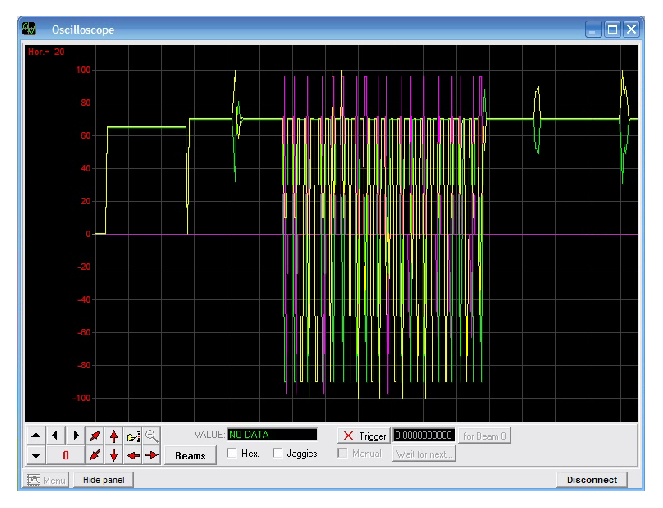
\includegraphics[scale=0.8]{figures/legonxt/oscilloscope.eps}
\caption[Bluetooth log diagram]{The bluetooth logger developed for windows. It has an interface similar
to an oscilloscope. It logs the signal of interest.
In this case the energy and the motor outputs.
 \label{nxtOsek:oscilloscope}}
\end{center}
\end{figure}

\subsubsection{How to guarantee real time operations?}
In Osek the task model is composed by 4 states as described in Fig.\ref{nxtOsek:taskModel}.
\begin{figure}[htbp]
\begin{center}
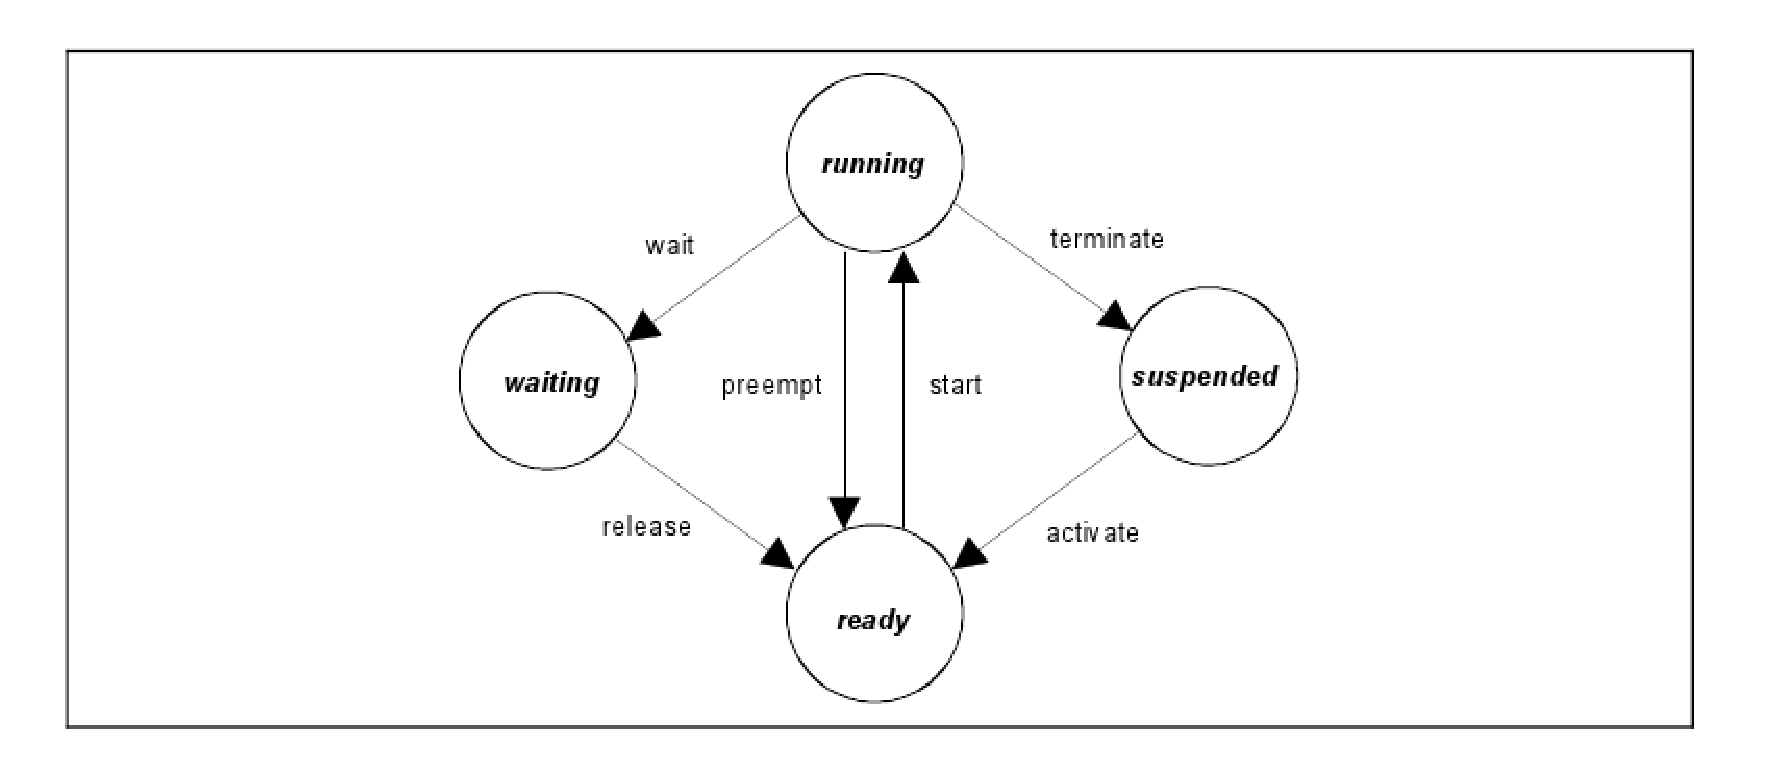
\includegraphics[scale=0.4]{figures/nxtosek/taskmodel.eps}
\caption[Real time task allocation]{A task must be able to change between several states, as the processor can only execute one
instruction of a task at any time, while several tasks may be competing for the processor at the
same time. The OSEK operating system is responsible for saving and restoring task context in
conjunction with task state transitions whenever necessary.
 \label{nxtOsek:taskModel}}
\end{center}
\end{figure}

A rate monotonic analysis is necessary to guarantee that for a particular application every task will be executed and completed in time. In Fig.\ref{nxtOsek:task} there's a simple explanation about how it works:
\begin{itemize}
 \item after the system boot all tasks are in ready state
 \item the task 4 with higher priority and is put in running state
 \item task 4 is terminated, the task with lower priority, 3, is put in running state
 \item after 10 ms task 4 is put again in run mode
 \item task 4 is terminated and task 2 is put in run mode
 \item task 1 is finally in run mode after task 2 is terminated
 \item nevertheless because task 4 with higher priority is due at 20 msec,
       task 2 is pre-empted (waiting state) in favour of task 4
 \item task 4 terminates and task 1 finishes etc.
\end{itemize}

Rate monotonic scheduling considers the 4 threads in the system and determines how much time is needed to meet the guarantees for the set of threads in question. It assumes that:
\begin{itemize}
\item No resource sharing (processes do not share resources, e.g. a hardware resource, a queue, or any kind of semaphore blocking or non-blocking (busy-waits))
\item Deterministic deadlines are exactly equal to periods
\item Static priorities (the task with the highest static priority that is runnable immediately preempts all other tasks)
\item Static priorities assigned according to the rate monotonic conventions (tasks with shorter periods/deadlines are given higher priorities)
 \item Context switch times and other thread operations are free and have no impact on the model
\end{itemize}

\citet{Liu73schedulingalgorithms} proved that for a set of $n$ periodic tasks with unique periods, a feasible schedule that will always meet deadlines exists if the CPU utilization is below a specific bound (depending on the number of tasks). The schedulability test is:

\begin{equation}
U=\sum_{i=1}^{n}\frac{C_{i}}{T_{i}} \leq n(\sqrt[n](2)-1).
\end{equation}

where $C_{i}$ is the computation time, and $T_{i}$ is the release period (with deadline one period later). For example $U = 0.8284$ for $n = 2$. When the number of processes tends towards infinity this expression will tend towards:
\begin{equation}
\lim_{n \rightarrow \infty} n(\sqrt[n](2)-1)=\ln(2) \approx 0.693147
\end{equation}
So a rough estimate is that RMS in the general case can meet all the deadlines if CPU utilization is 69.3\%. The other 30.7\% of the CPU can be dedicated to lower-priority non real-time tasks. It is known that a randomly generated periodic task system will meet all deadlines when the utilization is 85\% or less, however this fact depends on knowing the exact task statistics (periods, deadlines) which cannot be guaranteed for all task sets.
In my implementation in order to calculate $U$, $C_{1,2,3,4}$ must be computed using the Timer of the controller: execute every singular task individually and time it.
\begin{figure}[htbp]
\begin{center}
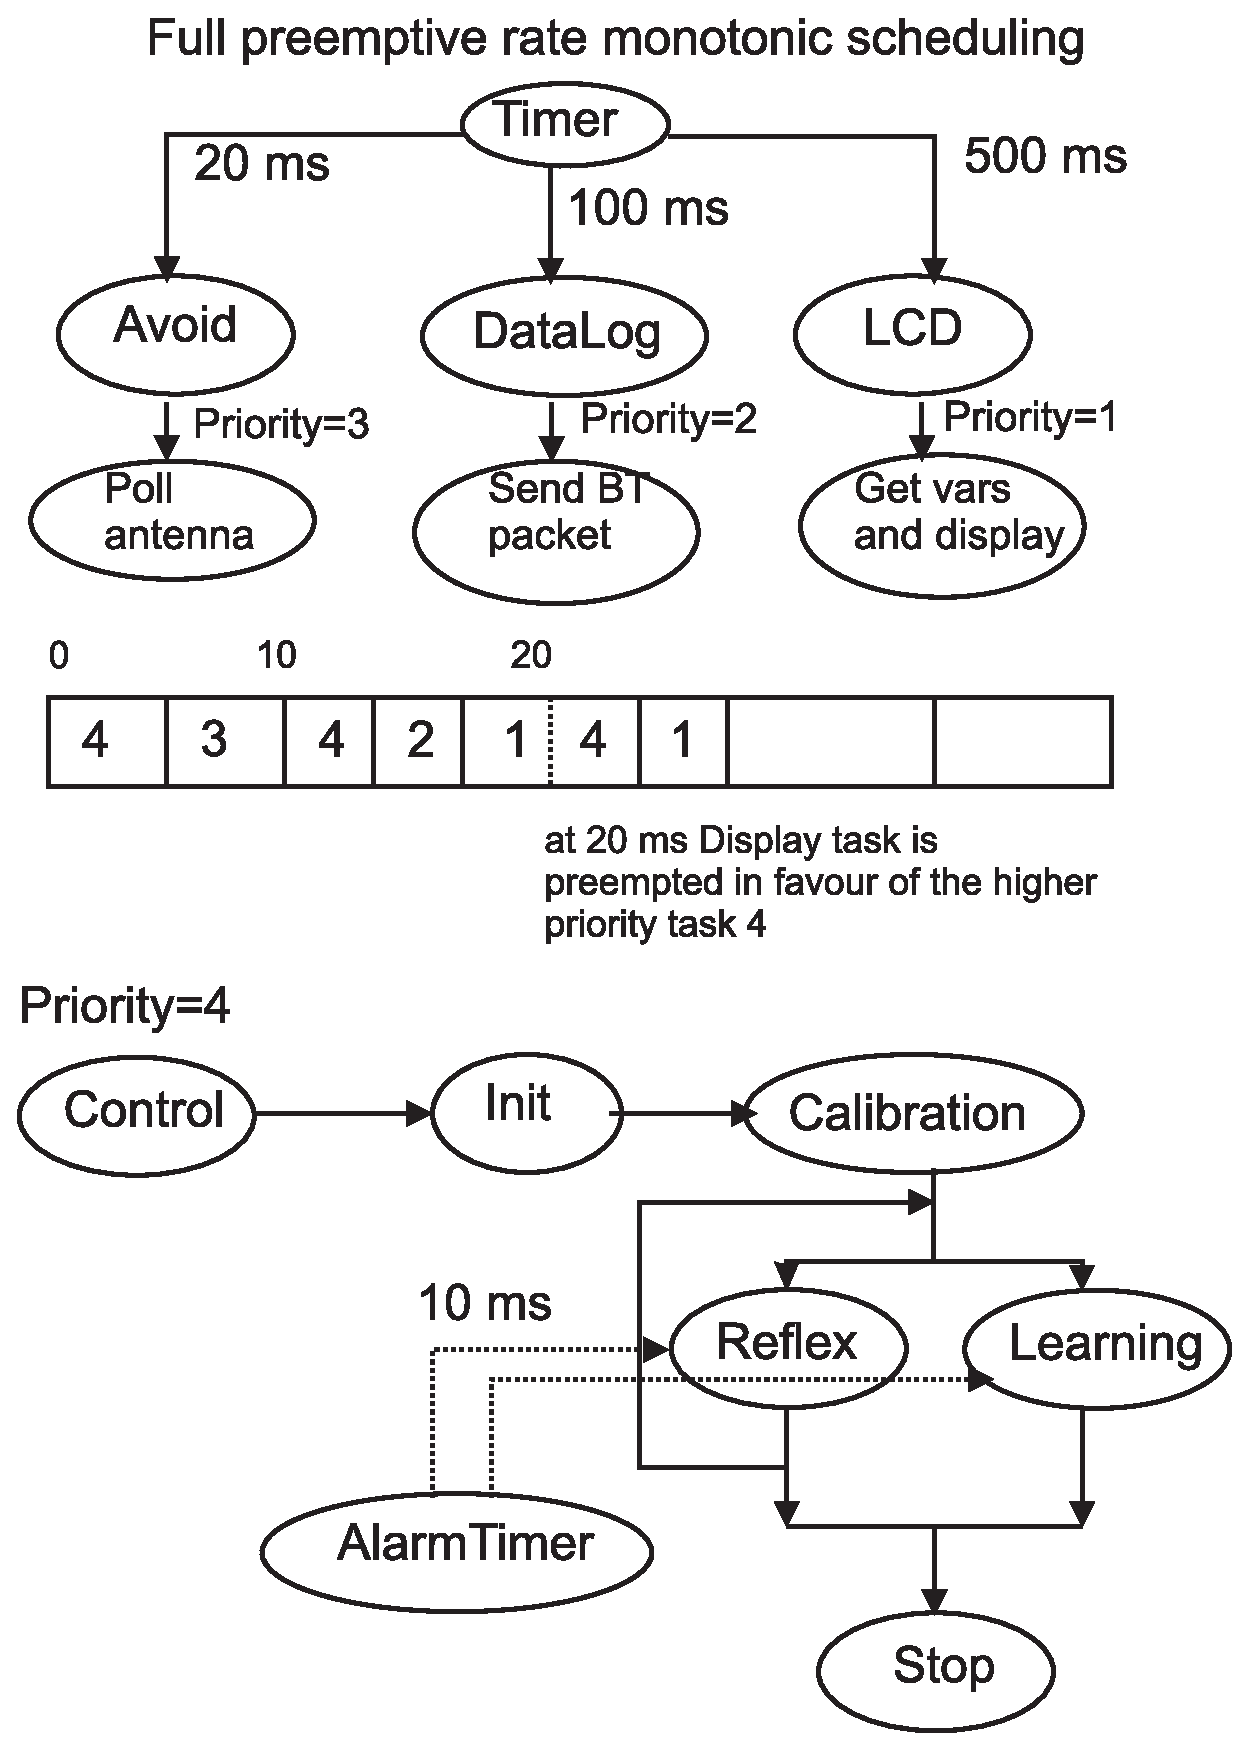
\includegraphics[scale=0.4]{figures/nxtosek/TaskLejos.eps}
\caption[Controller task allocation]{The control program task diagram.
There are 4 tasks scheduled in full-preemption mode. \label{nxtOsek:task}}
\end{center}
\end{figure}
\subsubsection{Communication and identification}
The most important aspect in our experiment is communication and identification.
We would like test 2 types of communication:
\begin{itemize}
 \item 1 to many: every agent broadcasts its state to everybody else
 \item 1 to 1: every agent communicates its state to a close peer
\end{itemize}

Communication is achieved by using the BluetoothCore and is structured as master-slave:
in a swarm slaves sends their phonemes (language primitives) to the master which has the role to dispatch them to the addressed receivers.
Every robot is identified by an ID which is inserted in every communication data packet. The packet is 32 byte long and its structure is in Fig.\ref{blue:communication}.
\begin{figure}[htbp]
\begin{center}
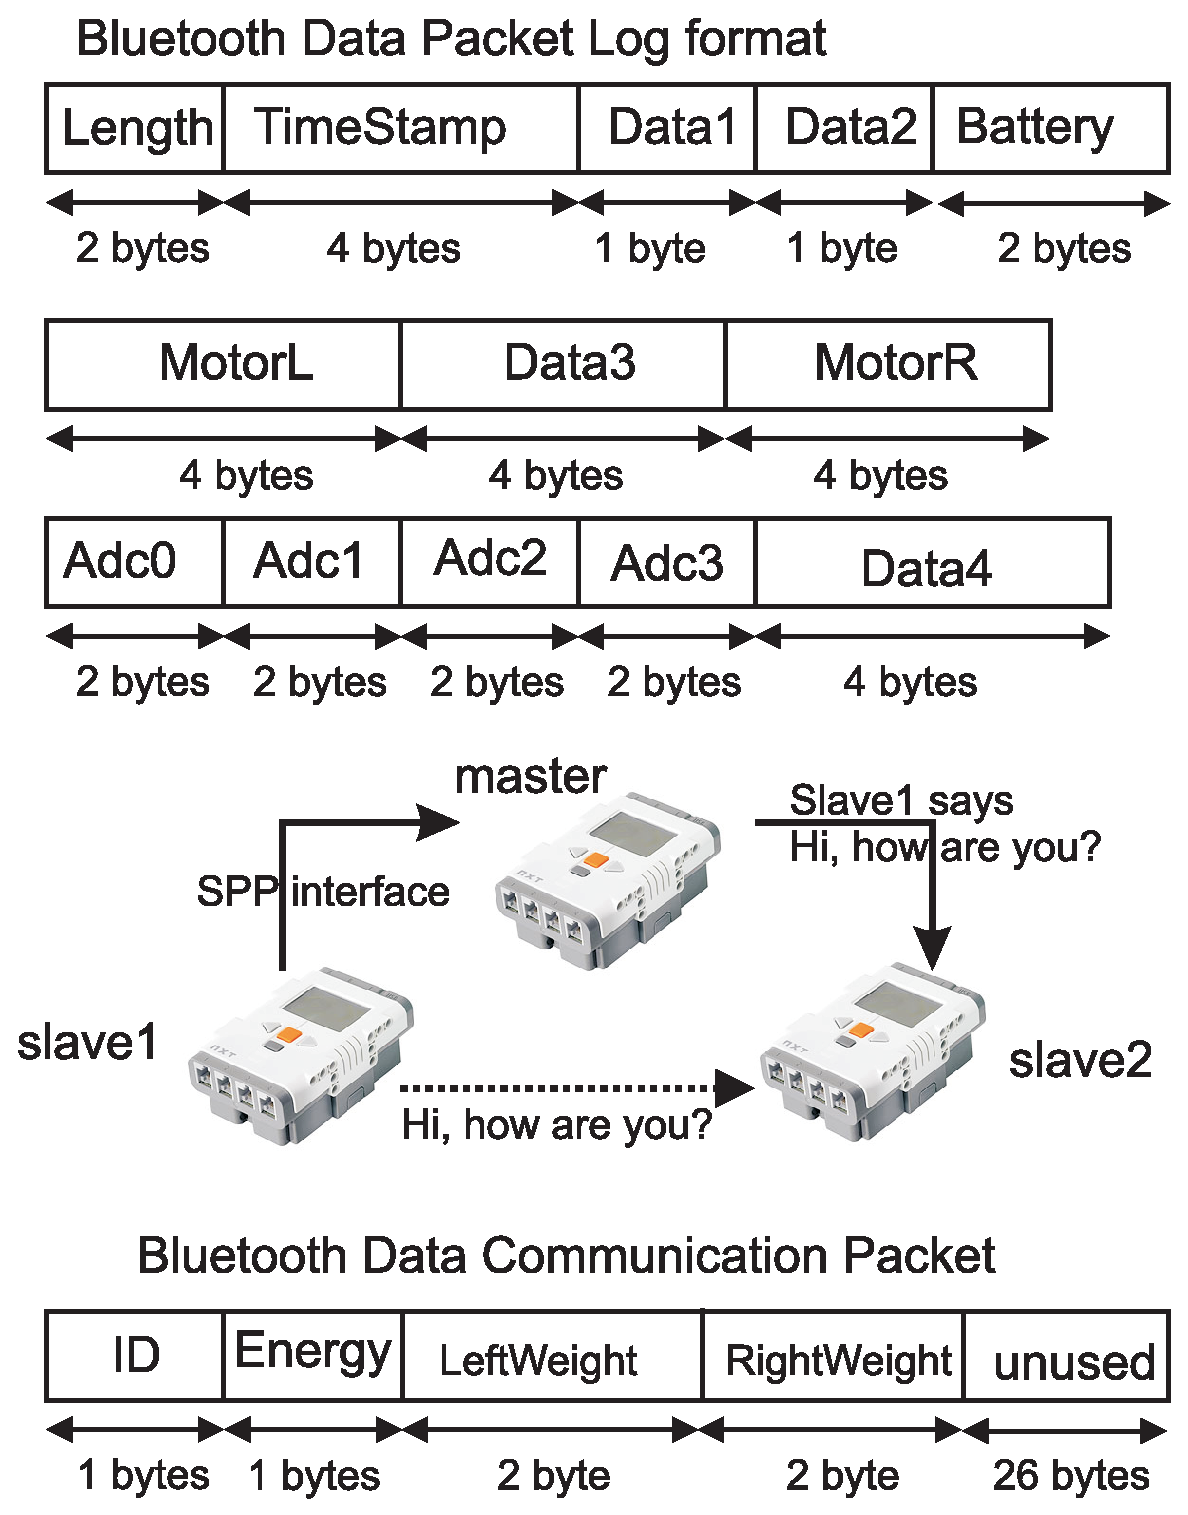
\includegraphics[scale=0.4]{figures/nxtosek/bluetoothlog.eps}
\caption{The bluetooth data logging structure.\label{blue:communication}}
\end{center}
\end{figure}
In this simple setup every robot is communicating its ID energy level to others.
The robot also communicates his energy level by producing a sound so that a human observer can have feedback about what's going on.
The lego speaker can play a tone, given its frequency, duration and volume. Frequency is audible from about 31 to 2100 Hertz and different frequencies are associated to different robots. The duration is in hundreds of a seconds (centiseconds, not milliseconds) and is truncated at 256, so the maximum duration of a tone is 2.56 seconds. The volume of the tone is proportional to the robot's energy which is normalised from 0 to 100 (internally is a float from 0.0 to 1.0).

\subsection{Pololu \label{Pololu}}

The Pololu 3pi \ref{Pololu}  robot is a complete, high-performance mobile platform featuring two micro metal gearmotors, five reflectance sensors, an $8x2$ character LCD, a buzzer, and three user pushbuttons, all connected to a C-programmable ATmega168 microcontroller. Capable of speeds exceeding 3 feet per second $(100 cm/second)$, 3pi is a great first robot for ambitious beginners and a perfect second robot for those looking to move up from non-programmable or slower beginner robots.
\textbf{Dimensions:}
Size: 	$9.5 cm/3.7"$ diameter,
\textbf{Weight:}
$83 g/2.9 oz$ without batteries
\textbf{General specifications}
\begin{itemize}
\item Processor: 	$ATmega168 @ 20 MHz$
\item Motor driver: 	TB6612FNG
\item Motor channels: 	2
\item User I/O lines: 	21
\item Minimum operating voltage: 	3 V2
\item Maximum operating voltage: 	7 V2
\item Maximum PWM frequency: 	80 kHz
\item Flash program memory: 16KB
\item Extra 512 bytes of persistent flash memory\footnote{is provided on the microcontroller for data logging or long-term learning applications}
\item Data memory: 1KB
\item Reverse voltage protection?: 	Y
\item External programmer required?: 	Y
\item
\end{itemize}
\textbf{Notes:}
\begin{enumerate}
\item Digital $I/O$ lines PD0 and PD1 are available; two more analog inputs and one analog/digital pin can be made available by removing jumpers and disabling special features of the board.
\item Designed for use with 4 x AAA NiMH or Alkaline cells. A step-up regulator boosts the motor voltage to 9.25 V.
\end{enumerate}

\begin{figure}[ht]
  \begin{center}
	\subfigure[Pololu robot bottom view: left and right light sensors]{
	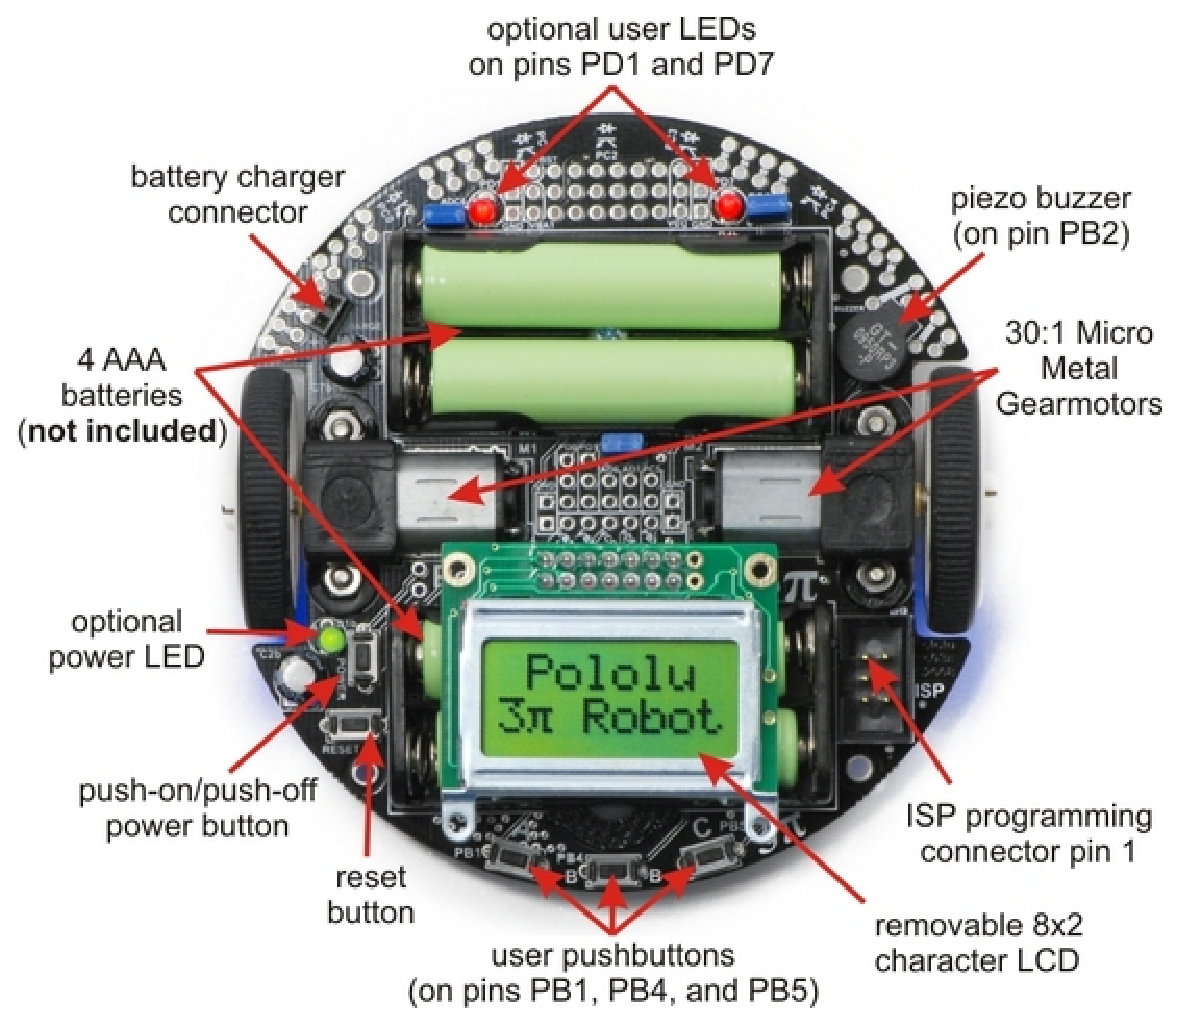
\includegraphics[scale=0.35]{figures/pololu/up.eps}}
	\hspace{1pt}
      	\subfigure[Pololu robot up view: left and right contact senros and LCD display]{
	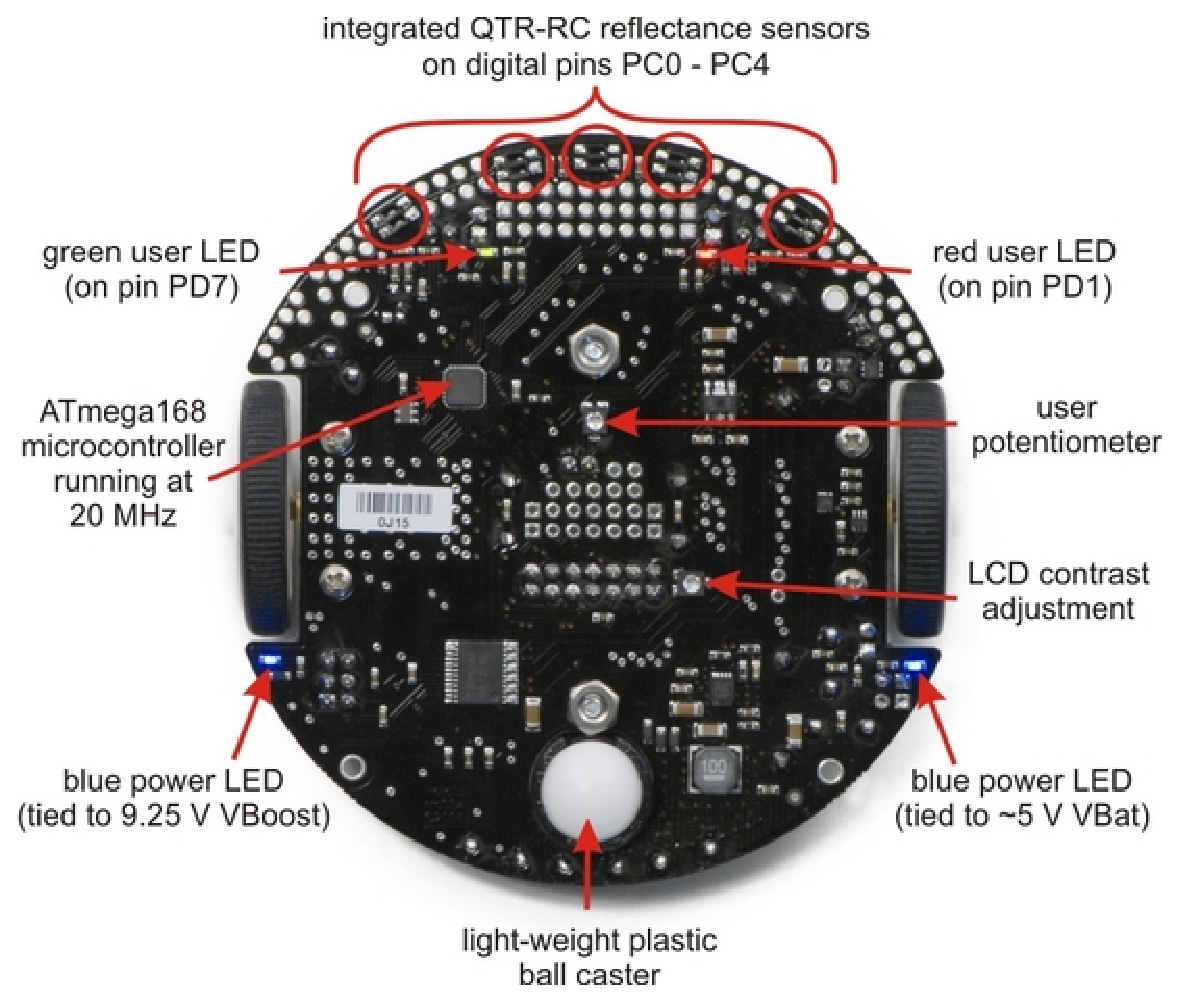
\includegraphics[scale=0.35]{figures/pololu/down.eps}}
  \caption[Pololu robot up and bottom view]{Pololu robot up and bottom view}
  \end{center}
\end{figure}
The processor is programmed using an external AVR ISP programmer such as the Orangutan USB programmer.
The popular, free GNU C/C++ compiler works perfectly with the 3pi, Atmel’s AVR Studio provides a comfortable development environment, and an extensive set of libraries provided by Pololu makes it a breeze to interface with all of the integrated hardware. The 3pi is also compatible with the popular Arduino development platform.

